\documentclass[11pt,oneside]{scrartcl}
 \usepackage[english]{babel}
\usepackage[applemac]{inputenc}
\usepackage[T1]{fontenc}
\usepackage{supertabular}
\usepackage{graphicx}
%\usepackage{flafter}
\usepackage{hyperref}
\renewcommand{\familydefault}{\sfdefault}
\usepackage{helvet}
\usepackage{rotating}
\usepackage[final]{pdfpages}
%\usepackage{hyperref}
\usepackage{listings}
\usepackage{supertabular}


%\setcounter{tocdepth}{3}
%\setcounter{secnumdepth}{3}
%\lstset{language=Perl}
\lstset{tabsize=2}
\lstset{frame=plain}

\setcounter{tocdepth}{1}

\begin{document}
{
\centering

\includegraphics[scale=0.2]{figs/logo.PNG}

~\\ 

{\noindent \huge \bf The friendly web framework\\~\\}
{\noindent \large \bf Programmers manual\\~\\}
{\noindent   Daniel B�hringer}

}
\tableofcontents
\newpage

\section{Introduction}
Desktop databases are perfect for rapid GUI prototyping. A major advantage is that  database rows are synced with the GUI automatically. However, most desktop database systems perform poorly under heavy load. Others are not suitable for programming web applications at all. 

<dbweb> is an Apache2-based web framework that provides rapid prototyping as well as deployment under heavy load. You can write a fully CRUD\footnote{Acronym for the basic operations operations create, update and delete}-functional web application with complex master detail semantics in (purely declarative) HTML-like syntax! 
Additionally, <dbweb> introduces specialized input elements such as ComboBox or DataGrid. These allow for handling very large data-sets as they fetch the data on demand and do not require  data pagination.

All application code (e.g. invoked from buttons, context menus) runs server-side\footnote{Currently, only Perl is supported, future releases may also support (server-side) Javascript}.
<dbweb> applications are nevertheless fully interactive and provide  confirm-dialogs or GUI-animation effects for immediate feedback. This is possible through Ajax technology. The Ajax-layer is hidden  to the  application developer by default.
An object oriented API provides access to the database through a thin object-relational mapper.

\section{Overview}
In <dbweb>, the GUI is written in HTML/CSS. <dbweb> introduces only a few additional tags (the most common are {\tt <foreach:..>... </foreach>}, {\tt <form:..>... </form>} and {\tt <var:..>}).  These tags always refer to  {\it DisplayGroup}s which connect the GUI to your databases. We discuss DisplayGroups  in chapter \ref{chap:dg}. 

Briefly, a DisplayGroup basically represents a single table/view in the database but additionally keeps track of row selection (a single row is always selected). The selection can be changed interactively or programmatically.  DisplayGroups can be connected to other DisplayGroups in master-detail configurations \footnote{\url{http://en.wikipedia.org/wiki/Master-detail}}. Commonly, a DisplayGroup feeds the data row-wise into a HTML table or a more specialized DataGrid view.

Data is edited within tables or through  dedicated forms. By default, all edits are immediately committed when the input element loses focus. All changes are reflected throughout  the GUI without page reloading.
DisplayGroups can also be enriched with context menus. Context-menus commonly trigger specific application code (chapter \ref{chap:coding}).

\section{Quickstart example}
\label{chap:quickstart}
We herein demonstrate how to write a simple data browser for a minimalistic two-table relational database. This database stores author-names together with their book titles (the SQL-schema is in listing \ref{lst:schema}). A screenshot of our finished application is in figure \ref{fig:form}. The user can change the selection of the authors table by left-clicking. The appropriate book titles automatically show up next-by. Changes are immediately committed upon editing the form. The GUI elements update without page reloading.

\begin{figure}[htbp]
\centering
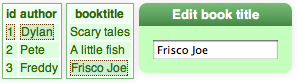
\includegraphics[scale=0.8]{figs/editing.PNG}
\caption{Screenshot of our data browser for the authors/books database \ref{lst:form}. The first author is selected (dotted border). The second column lists only the books of that author. A particular book is selected and can be edited in the form to the right.}
\label{fig:form}
\end{figure}


The <dbweb> code for figure \ref{fig:form} is in listing \ref{lst:form}. The data tables and the form are laid out column-wise (lines 1-4). Lines 5-16 comprise the author-table. This table is generated through the concept of {\it foreach repetition} (discussed in detail in section \ref{chap:foreach}).
Briefly, a template (lines 11-14) is concatenated for each data-row in the DisplayGroup {\tt authors} (line 10). The two {\tt var:...} tags are substituted by the appropriate content in each row. The same concept applies to the book-title table (lines 19-28). This table automatically displays only the appropriate rows, depending on the selection of the first table.
The rightmost column comprises of a form (lines 31-33). This form allows for editing the current book title (line 33). See chapter \ref{chap:forms} for a full discussion of forms. 

But how does <dbweb> know which are the appropriate book-records are to be listed in the books-table? Where is the information the database connection? These informations are bundled in the DisplayGroups, that also keep track of the selected rows.  Listing \ref{lst:dg} gives the DisplayGroup code for our example. This code is commonly auto-generated from the SQL-schema, so you should not worry about the complexity at this stage.


The <dbweb>-Apache2-module transparently transforms the 37 lines from listing \ref{lst:form} into plain HLML and Javascript that works with all current web-browsers. All tables are click-responsive and the detail form is automatically connected to the master table. This is interesting, because we did not write any code for event processing or database access. 
Obviously, <dbweb> factors away all tedious event processing code. A similar AJAX application written e.g. directly in Javascript and a server-side scripting language such as perl/PHP would span at least 1000 lines of  code even for our simple example scenario. The complexity comes from cross-browser compatibility and the edge cases such as changing selection during editing.


\begin{lstlisting}[caption=Complete source code of our authors and book example. <dbweb>-keywords are in boldface.,  label= lst:form, basicstyle={\small\ttfamily}, numbers=left]
<html>
<table>
<tr>
<td valign=top>
	<table class="datatable">
		<tr>
		<th>id</th>
		<th>author</th>
		</tr>
		<foreach:authors>
		<tr>
			<td><var:id></td>
			<td><var:name></td>
		</tr>
	</foreach>
	</table>
</td>
<td valign=top>
	<table class="datatable">
		<tr>
		<th>booktitle</th>
		</tr>
		<foreach:books>
		<tr>
			<td><var:title></td>
		</tr>
		</foreach>
	</table>
</td>
<td valign=top>
<form:books format:label="Edit book title">
	<var:title edittype=text>
</form>
</td>
</table>
</body>
</html>

\end{lstlisting}



\section{GUI programming}
\subsection{Foreach repetition}
\label{chap:foreach}

The most basic way to expose database content tabularly is {\it foreach repetition}. E.g.  the template of a  HTML table row is concatenated for each data-row in the DisplayGroup from the enclosing {\tt foreach}. Chapter  \ref{chap:quickstart} gives a basic example.


\noindent The  generalized syntax is:
 {\tt <foreach:{\it DG[.filterName][options]}>} ...  {\tt </foreach>}  where {\it DG} is the name of any DisplayGroup, {\it options} an optional set of parameters (table \ref{tab:foreachpars}). The enclosed template block is commonly the template for a single table row. Herein, database values can be exposed through {\tt <var:..>} tags (see next section). The filterName option is discussed in chapter \ref{chap:filtering}\\


\begin{table}[htdp]
\caption{Parameters of the {\tt foreach} tag. }
\begin{center}
\begin{tabular}{p{3.5cm}p{10cm}}
Parameter & Description\\\hline
plain=YES & Performs template processing only without making the rendered table interactive. This option is only useful in very advanced setups. With this option set, automatic user interaction and standard master-detail set-ups will not work as advertised. \\
classnameVar={\it col}& This option will assign a CSS classname by textually concatenating {\tt class}, {\it col} and the acutal value of {\it col} for the current row. You can use this feature to automatically highlight rows on the basis of a certain value in the current row. You can define the highlighting style in your CSS (see chapter \ref{chap:modularizing} for where to placing the CSS).\\
perl={\it perlfuncName}& {\it perlfuncName} is invoked in each iteration and can modify the template processing.\\
\end{tabular}
\end{center}
\label{tab:foreachpars}
\end{table}

\noindent  Apart from rendering <dbweb> tables to pure HTML,  {\it foreach repetition} additionally makes the resulting HTML table interactive by default: the user can change the selected row by clicking on the table.
<dbweb> ensures that the elements of the selected row are automatically assigned to the CSS class {\tt selectedRow} in the web browser. The default <dbweb> stylesheet defines a slightly darker background colour and a dotted border. The visual results are best when the table is assigned the CSS-class  {\tt datatable}. 


\subsection{Exposing database content}
Database content is exposed through {\tt <var:}{\it column name}{\tt>} tags. These tags are only meaningful within {\tt <foreach:>} or {\tt <form:...>} environments that connect the column names to the appropriate database tables through a DisplayGroup.
\noindent The  generalized syntax of the {\tt <var:>} tag is:
 {\tt <var:}{\it column name} [{\it options}]>  where {\it column name} is the name of a valid column in the DisplayGroup referred to by the surrounding  {\tt <foreach>} or {\tt <form>} environments. {\it options} an optional set of parameters discussed in table \ref{tab:varpars}.\\

\begin{table}[htdp]
\caption{Common parameters for the {\tt var:} tag. Additional options are discussed in table \ref{tab:edittypes} together with the respective  edittypes.}
\begin{center}
\begin{tabular}{p{3.5cm}p{10.5cm}}
Parameter & Description\\\hline
edittype={\it aType}& This option makes the data editable and also determines the input element. {\it aType} is one of   {\tt  text, password, plain, combo, popup, boolean, textarea, button} and {\tt upload}. See table \ref{tab:edittypes} for a detailed discussion of these edittypes.\\
class="{\it aCSSclass}" & Adds {\it aCSSclass} to the input element int the DOM. \\
style="{\it aStyle}"& The CSS-style of the input element is set to {\it aStyle}.\\
id="{\it aDOMid}"& Assigns the {\it aDOMid} to the input element. You can refer to the input element in your custom JavaScript. You are responsible to ensure that  {\it aDOMid} is unique in the DOM. \\
autocomplete="off"& Turns off the autocompletion feature built into the modern browsers. \\
format:label="{\it aLabel}"& {\it aLabel} is translated to a HTML label tag assigned to the resulting input element.\\
format:date="{\it format\-string}"& Translates calendarial database content to UI representation and vice versa through a POSIX date format string. E.g. in Germany, dates are commonly formatted {\tt \%d.\%m.\%Y} whereas the format-string of the ISO standard is {\tt \%Y-\%m-\%d}. Please refer to the  {\tt date} manpage of your web server  system for all date-component tokens that are available on your system.\\
format:typeahead= "{\it DG.col}"& Pulls down a pick-list below the input control upon typing just like  the autocomplete feature of modern web-browsers. However, this option limits the autocompletion list to the data from column {\it col} of DisplayGroup {\it DG}.\\
format:lookup= "{\it DG.col}"& Substitutes the value of the column specified by <var:...>  (current column) with the value of {\it col} in DisplayGroup {\it DG}. The value is taken from the row in DG whose primaryKey equals the value of the current column value (just like in SQL joins).\\
\end{tabular}
\end{center}
\label{tab:varpars}
\end{table}

\begin{table}[htdp]
\caption{Discussion of all edittypes for the {\tt var:} tag.}
\begin{center}
\begin{tabular}{p{4cm}p{10cm}}
Parameter & Description\\\hline
text, password& Single line text input (masked for password). This width of the input field can be modified with the option {\tt size="{\it countColNums}"} with {\it countColNums} a numeric value that has to be optimized empirically.\\
textarea& Multiline text input. Width and height of the input area are specified through the   {\tt width="{\it countColNums}"}  and {\tt height="{\it countRowNums}"} options, respectively.   \\

plain& Substituted by the data without any transformations.\\

popup, combo& Edit a foreign key on the basis of a   (more user friendly) surrogate column. Popup provides a {\it select} input element, combo renders to a single line text input element with an Ajax-pick-list attached below. Use popup if the list is rather small. Use combo for larger lists as the options are constantly narrowed during typing. Large pick-lists may slow down the browser significantly after focussing the combo element. Here, {\tt format:pulldown="off"} can prevent the complete pick-list to pull down initially. The  {\it surrogate column}  from DisplayGroup {\it DG} is determined through {\tt format:data="{\it DG.surrogateColumn[.filterName]}"} for both popup and combo. The primaryKey of {\it DG} rather than the surrogate column is bound to the associated {\tt var} tag. The option {\tt  format:notNull="YES"} ensures that the first entry from the data-source is preselected (instead of the NULL value) and that no  empty (NULL) option is available in the popup/pick list.\\
boolean& Checkbox for boolean data. Note that NULL and FALSE cannot be distinguished by the end-user. \\
button & Button input element. Server-side code can be attached through {\tt perlfunc="{\it aPerlFuncName}"}. See chapter xx for where to put the server-side code.\\
upload& Provides an Ajax-powered upload button to directly place the data from client-side files into the database.\\
\end{tabular}
\end{center}
\label{tab:edittypes}
\end{table}

\subsection{Editing Data through forms}
\label{chap:forms}
Forms group related data for editing. The form data is automatically bound to --- and kept in sync with the selected row of the form's DisplayGroup. The selected row can e.g. be changed by clicking at a table that is bound to the same DisplayGroup.
Listing \ref{lst:form} and figure \ref{fig:form} give a basic example of a simple form that also demonstrates some of the {\tt var} tags discussed in the previous section. The full syntax is:
 {\tt <form:{\it DG} [{\it options}]> ...</form>} where {\it DG} is the name of any DisplayGroup and {\it options} an optional set of parameters (table \ref{tab:formpars}). The enclosed part typically comprises of {\tt <var:..>} tags with the edittype attribute set appropriately (see previous section).\\


\begin{table}[htdp]
\caption{Parameters of the {\tt foreach} tag. }
\begin{center}
\begin{tabular}{p{3.5cm}p{10cm}}
Parameter & Description\\\hline
label="someLabel" & Adds someLabel as heading above this form. \\
style="someCSS" & Adds someCSS the the CSS style of this form. \\
id="someID" & Assigns DOM-id {\it someID} to this form. \\
plain=YES & Transforms to pure HTML form without <dbweb> mechanics. \\
perl={\it perlfuncName}& {\it perlfuncName} is invoked upon data editing for validation. See section xx.\\
\end{tabular}
\end{center}
\label{tab:formpars}
\end{table}

\subsection{DataGrid Tables}
\label{chap:datagrid}

The major drawback of {\it foreach repetition} is that the page may get very large when the DisplayGroup holds more than 50 rows. This would hamper usability and speed in the Web browser. DataGrid Tables provide a scroll bar to a fixed height table and fetches only the currently visible subset of rows from the database. This allows for displaying arbitrary long tables without pagination.
The  generalized syntax is in listing \ref{lst:table}.

\begin{lstlisting}[caption=Syntax-block for DataGrids (see chapter \ref{chap:sorting} for a discussion of the optional filterName attribute), label=lst:table, basicstyle={\small\ttfamily}]
	<table:someDG[.filterName] rows="CountOfVisibleRows">
		<head>
			<col:WidthOfColumn> SomeHeaderName </col>
			<col:WidthOfOhterColumn> OtherHeaderName </col>
		</head>	
		<foreach>
			<cell><var:columnName></cell>
			<cell><var:otherColumnName></cell>
		</foreach>
	</table:someDG>
\end{lstlisting}

\noindent where {\it columnName} and {\it otherColumnName} are valid columns in Display\-Group {\it some\-DG}. The visible height of the table is set through the integer {\it CountOfVisibleRows}. The table appearance is identical to foreach repetition If the row count is lower or equal to this value. Otherwise, a native scrollbar is attached to the right of the table. The column with is fixed. Oversized cells are clipped. The column.width is pre-set in the header section through {\it WidthOfColumn} and {\it WidthOfOhterColumn}. These values have to specified as integer postfixed by unit, such as {\tt 110px} for 110 pixels width in the browser layout.\\

\subsection{Conditions in the User Interface}
Parts of the UI can be conditionally hidden away on the basis of database-values. Typical uses for conditional parts of the UI is to hiding elements that does not make sense in a particular context. Another usage is to  implementing tabs that structure large forms into smaller aspects of semantically related fields.

In <dbweb>, conditional parts of the UI are placed within the {\tt <cond var:...>} and  {\tt <condDG:...>} environments.
\noindent The former construct is valid only within a  {\tt <foreach:...>} or {\tt <form:...>} environment that provides the link to a DisplayGroup. Here, the formal  syntax is:
 {\tt<cond var:}{\it columnName} {\tt=}{\it condition}{\tt>} ... {\tt</cond>}
\\\noindent where {\it column name} is the name of a valid column in the DisplayGroup referred to by the surrounding  {\tt <foreach:...>} or {\tt <form:...>} environments. {\it condition} is discussed in table \ref{tab:condpars}.

{\tt<condDG:}, the other incarnation of conditionals can be placed anywhere as the DisplayGroup is specified with the tag. The syntax is:

\noindent {\tt<condDG:}{\it aDG} {\tt var:}{\it columnName} {\tt=}{\it condition}{\tt>} ... {\tt</condDG:}{\it aDG>}
\noindent with aDG the DisplayGroup whose columnName of the selected row is queried against the condition.



\begin{table}[htdp]
\caption{Syntax for condition statements. The enclosed block is deleted during rendering unless the condition evaluates true. The selection and count keywords are valid only for  {\tt<condDG:}... environments.}
\begin{center}
\begin{tabular}{p{6cm}p{8cm}}
var:columnName= & True if data...\\\hline
const:{\it someLiteral} & ...equals to {\it someLiteral}\\
eq:const:{\it someLiteral} & ...equals to {\it someLiteral}\\
ne:const:{\it someLiteral} & ...is not equal to {\it someLiteral}\\
gt:const:{\it someLiteral} & ...is greater than {\it someLiteral}\\
lt:const:{\it someLiteral} & ...is less than {\it someLiteral}\\
eqnull & ...is a NULL value (in database sense)\\
nenull & ...is not a NULL value (in database sense)\\\hline\hline
selection= & True if selection...\\\hline
true & ...is true in boolean context\\
false & ...is false in boolean context\\
visible & ...is visible\\
invisible & ...is invisible\\
empty & ...is empty\\\hline\hline
count= gt:const:{\it someNumber} & True if the DisplayGroup holds more rows than {\it someNumber}.\\
\end{tabular}
\end{center}
\label{tab:condpars}
\end{table}



\section{Database interface}
\label{chap:dg}
\subsection{What is a DisplayGroup?}
DisplayGroups encapsulate database tables/ views for <dbweb>. A DisplayGroup represents a single database table/view one-by-one. However, it additionally keeps track of a selected row. The first row of the DisplayGroup (in the database order, unless you supply ordering specifications, see section \ref{chap:ordering}) becomes selected during initialization. The selection can be changed interactively by the user through clicking at any row, or programmatically through the API. 

By default, DisplayGroups hold the full dataset of the underlying database table. These DisplayGroups are called {\it master} DisplayGroups and need a connection-property to make the link to the database (see table \ref{tab:dg1}). DisplayGroups can also be connected to other  DisplayGroups by means of  the {\tt bindToDG} property. These connected DisplayGroups inherit the database connection from their master DisplayGroup. They can additionally be configured to become a {\it detail} DisplayGroup  through providing the {\tt bindFromColumn} property. {\it Detail} DisplayGroups hold only the subset of all rows with the foreign key from the bindFromColumn property  equalling  the primary key of the  selected row in their master DisplayGroup. In our  author-book example application (figure \ref{fig:form}) the authors DisplayGroup is the master DisplayGroup and the books DisplayGroup is configured as a detail DisplayGroup. 

DisplayGroups are declared within the {\tt <DisplayGroup {\it [options]}}... {\tt </DisplayGroup>} environment. {\it [options]} specifies the syntax of the enclosing display group definitions. Multiple <DisplayGroup> environments can be declared within a single file or   included from library files, see section \ref{chap:modularizing}. <dbweb> supports JSON and classical Apple PropertyList syntax. The latter is the default, JSON has to be marked out by {\tt format="JSON"}. All examples in this document are in Apple PropertyList syntax as this markup language is much easier to read.


\subsubsection{DisplayGroups for database tables}
Our minimalistic relational database from the introduction example is shown in SQL syntax  in listing  \ref{lst:schema}. The corresponding DisplayGroup definition is given in listing  \ref{lst:dg}. Table \ref{tab:dg} and \ref{tab:dg1} list all properties of a DisplayGroup.

\begin{table}[htdp]
\caption{Basic DisplayGroup properties. You may want to use ModelMaker.pl to generate the markup directly from SQL-syntax.}
\begin{center}
\begin{tabular}{p{4cm}p{10cm}}
Property & Explanation\\\hline
table & Name of the database table.\\
columns & List of all column names that are made accessible from the table.\\ 
primaryKey& Name of the primary key of table. {\bf Note:} Only primaryKeys with values exclusively made of digits, a-z (case insensitive), whitespace, dots and underscore characters are currently supported by <dbweb>.\\
types & Key-Value dictionary specifying the database types (values) of all non-text columns (keys). Valid types are bool, int (also valid for floats) and date (also valid for timestamps). \\ 
write\_table & Optional name of a database table for writing, e.g. when table points to a read-only view. Newer versions of PostgreSQL require the type specification. May be optional in other settings.\\
suppress\_insert & Optional list of columns that are not valid within write\_table. Otherwise  database errors will occur upon inserts and updates.\\
connection & Dbi-DSN specifying the database connection. When omitted, the DisplayGroup chain (see boundToDG property) is iterated for the connection.\\ 
connectionEnv & Name of an environment variable holding the connection string (useful when switching from a test- to a production without modifying the source code).\\ 
connectionEnvAuto & When set to YES, the connectionstring is taken from the environment variable with name {\tt dbweb\_connection\-string\_}{\it nameOfYourApp}.\\ 
user, password & Database credentials for the connection (optional, see chapter \ref{chap:security}).\\ 
encoding & Encoding of the database table (defaults to latin1).\\
\end{tabular}
\end{center}
\label{tab:dg1}
\end{table}

\begin{table}[htdp]
\caption{Advanced DisplayGroup properties.}
\begin{center}
\begin{tabular}{p{4cm}p{10cm}}
Property & Explanation\\\hline
boundToDG & Name of the parent DisplayGroup\\
bindFromKey & Name of the foreign key column in this DisplayGroup\\
targetColumn & Name of the binding key in the master DisplayGroup. Defaults to the primaryKey in the master DG if omitted.\\
data & See section \ref{chap:sdg}\\
cache & Copies {\it all} rows from table into the session. Subsequent reads come from the cache that is synced with updates from <dbweb>. Useful for working with long-loading complex views. Do not use with long-tables as this would slow down the current session. See also section \ref{chap:cache}\\
DataInSession & Hold global variables. See section \ref{chap:dis}.\\
contextmenu & Define a context menu. See section \ref{chap:cm}.\\
autoSort, sortColumns& Specify sorting of the data. See section \ref{chap:sorting}.\\
filters& Specify filters that can be accessed from the UI layer. See section \ref{chap:filtering}.\\
\end{tabular}
\end{center}
\label{tab:dg}
\end{table}


\begin{lstlisting}[caption= SQL schema of a minimalistic relational example database.  (PostgreSQL syntax), label=lst:schema, basicstyle={\small\ttfamily}]
CREATE TABLE authors ( 
    id    serial PRIMARY KEY, 
    name  varchar
); 

CREATE TABLE books ( 
    id          serial PRIMARY KEY, 
    author_id   int4 references authors(id), 
    title       varchar
); 
\end{lstlisting}

\begin{lstlisting}[caption= DisplayGroup markup of the SQL from listing \ref{lst:schema}. Please refer to table xx for a discussion on secure ways to provide the connection string and database credentials.,  label=lst:dg, basicstyle={\small\ttfamily}]
	authors = {
		table="authors";
		columns = ( id, name );
		types = { id = int; };
		primaryKey = id;
		connection="dbi:Pg:dbname=test;user=root;host=localhost";
	};
	books = {
		table="books";
		columns = ( id, author_id, title );
		types = {id = int; author_id = int; };
		primaryKey = id;
		bindToDG="authors"; bindFromColumn="author_id";
	};
\end{lstlisting}


\subsubsection{DisplayGroups for static data}
\label{chap:sdg}
Data can also directly placed in the DisplayGroup. This is useful for feeding Tab-controls. See Listing \ref{lst:static}.
\label{lst:staticdg}
\begin{lstlisting}[caption= The data is statically attached in this basic example, basicstyle={\small\ttfamily}, label=lst:static]
<DisplayGroups>
{	myDG = {
		columns = ( id, name );
		types = { id = int; };
		primaryKey = id;
		data = ((1,"Pictures"),   (2, "Pictures Long"),
						(3, "Features" ), (4, "Relatives" ) );
	};
}
</DisplayGroups>
\end{lstlisting}

\subsubsection{DisplayGroups for global variables}
\label{chap:dis}
Global variables of the current session is best kept in a DisplayGroup with the DataInSession=YES attribute. This DG has only a single row that is always selected. The data is stored in the current session.

\subsubsection{DisplayGroups for in-memory data}
\label{chap:cache}
Data not from databases is handled in display groups with the Cache=YES attribute and no table attribute. The data has to be pumped in through the API and is stored in the current session.

\subsubsection{DisplayGroups for Cookies/ HTML5-storage}
This is not yet implemented but may be supported in future releases if there is user-demand arises.

\subsection{Sorting}
\label{chap:sorting}
By default, dbweb does not sort data but preserves the order returned from the database. This conservative behaviour can be overridden through the {\tt autoSort} and {\tt sortColumns} properties of a DisplayGroup. The sortColumns property specifies a hash of column names as illustrated in listing \ref{lst:sorting}. You can depose further sorting policies under different names but retrieving them is currently unsupported.

\begin{lstlisting}[caption=Syntax for automatic sorting. This DisplayGroup will contain that are primarly sorted for Column1 and secondarily by Column2,  label= lst:sorting, basicstyle={\small\ttfamily}]
someDG={
	...
 	autoSort="mySortingSpec";
	sortColumns=
	{	mySortingSpec =("Column1", "Column1");
		otherSortingSpec =("Column2", "Column1");
	};
};
\end{lstlisting}


\subsection{Filtering}
\label{chap:filtering}
Filters specify different subsets of the full DisplayGroup dataset. You can select filters in the  {\tt <foreach>} (chapter \ref{chap:foreach}) or  {\tt <table>}  (chapter \ref{chap:datagrid}) environments, and also in datasource attributes of popup/combobox GUI elements (table \ref{tab:edittypes}).
Filters are static by default. You can only specify constant attributes. However, you can modify filters at runtime, e.g. in the \_earlyauto\_ event handler. Here, you can e.g. overwrite the constant val attribute of  a certain filter-element (listing xx). This is e.g. useful for only displaying the records, that the current user is allowed to see. The property name for filters is {\tt filters}. The basic syntax for filters is very similar to sorting (chapter \ref{chap:sorting}). The filters hash holds condition arrays. A single condition has this form: {\tt \{col="someCol"; op="someOperator"; val="someValue"\}}. The condition is only true if all condition elements are true (logical AND). someOperator can be  eq, ne, eqnull, nenull or literal. The val property can be omitted for eqnull and nenull, that test for NULL or non-NULL (in database speaking), respectively. A valid SQL fragment is required in the val property for the literal operator, a constant value otherwise.

\subsection{Context menus}
\label{chap:cm}
Context menus provide specific actions that may be tailored the the data in a specific DisplayGroup. For this reason, each  DisplayGroup can have its own context menu. The context menu opens upon right clicking any row that belongs to this DisplayGroup. The context menu is configured through the {\tt contextmenu} property of a DisplayGroup. Like a filter, this hash contains arrays of entry elements. A single entry element has this form:

\begin{lstlisting}[caption=Context menus are defined in the DisplayGroup. You can add separators or  invoke perl code or perform simple DOM manipulations such as unhiding a GUI element,  label=lst:cm, basicstyle={\small\ttfamily}]
someDG={
	...
	contextmenu=
	(	{	name="Selektieren";
			action="select";
		}, { separator="true"; },
		{	name="Bestaetigen";
			raiseDOMId="dom_opdat";
		},
		{	name="OP geht nicht";
			perlfunc="enter_blockdate";
		}
	);
};
\end{lstlisting}


\section{Application partitioning and navigation}
\label{chap:modularizing}
Web applications are commonly split into (full-screen) sub-applications that cover specific sub-domains of the application. E.g. one page could cover customer administration whereas an other  page could handle user-admin issues. Commonly, a fixed navigation element visually groups these sub-application to a single 'application-cluster'.
<dbweb>-application-clusters usually reside in a cluster-specific subdirectory below dbwebressources (as defined in your httpd.conf, Listing \ref{lst:install}, lines 3 and 4).

When an URL requests a path below your dbweb URL-location (in your httpd.conf, see Listing \ref{lst:install}, line 5)  such as {\tt http://localhost/dbweb/myapp}, <dbweb> automatically jumps to the page called login.dgwapp inside of directory {\tt myapp}. This file has to always  exist. This behavior can be overriden through a t=targetApp in the URL. Simple authentication-free applications can be written within login.dgwapp. However, this page typically redirects to the main application page of the application cluster upon sucessful authentication through the API.
Each dgwapp can have it's own CSS with the same name but css extension instead of dgwapp. A common CSS is automatically read from style.css below your dbwebressources.



\subsection{Jumping between dgwapps}
This is accoplished through <link:someTarget> tags.
\subsection{Navigation tabs}
You should include a common header that provides...

\section{Application programming}
\label{chap:coding}
Commonly, applications comprise of functionality beyond the basic CRUD operations and database navigation. E.g. reporting tools may download a PDF or an email should be sent when a button is pressed. Such application specific code is  is organized in functional units named perlfuncs for historical reasons. A perlfunc can be semantically regarded a subroutine containing arbitrary code. This code is executed by the same version of perl as in the the mod\_perl2 of your web server. Perlfuncs reside inside the dgwapp inside the {\tt <perlfunc..>} environment.  
The syntax definition is given in Listing \ref{lst:simpleperlfunc}.

\begin{lstlisting}[caption=Syntac for perlfunc definition. SomeFile is commonly a perl library relative to dbwebressources.,  label=lst:simpleperlfunc, basicstyle={\small\ttfamily}]
<perlfunc name=someName" include="SomeFile">
{	....
}</perlfunc>
\end{lstlisting}

Perlfuncs  may be hooked to buttons and context menus through the {\tt perl=} and {\tt action=}  keywords, respectively. Perlfuncs can also be automatically invoked at various places within the event loop or upon data updates or inserts. The code is executed inside a specialized environment, with all a perl-object instantiated for each DisplayGroup below the {\tt \$DG::} namespace. See section \ref{chap:api} for a discussion of these objects' methods and other functions to manipulate the application state, UI and database.


\subsection{Refactoring}
A central element for factoring out your common code-components is the include statement.
The syntax for including is:

\noindent {\tt <include src="path/local/to/dbwebressources.dgw">}\\
\noindent the extension can be chosen freely, dgw is only a convention. <html> and <DisplayGroup> environments are merged into the current application as well as all <perlfuncs>. The code is concatenated in case a perlfunc of the same names is already defined in the current application. This is useful e.g. for refacturing authentification checks out of application-specific \_auto\_ or \_earlyauto\_ handlers.
%<!>talk about the power of linking in code from perl modules (stefan?)

\subsection{API}
\label{chap:api}
Explain basic stuff like DG namespace, undef and NULL, encoding issues

\begin{table}[htdp]
\caption{DisplayGroup methods for basic database operations.}
\begin{center}
\begin{tabular}{p{5cm}p{9cm}}
\$DG::someDG->... & Explanation\\\hline
insertDict(\$aDictRef); & Inserts \$aDict into the database table referenced by someDG. Returns the value of the primaryKey for the newly inserted row. Keys of \$aDict not corresponding to valid column names are ignored. \\
insertDictUsingFilter(\$aDictRef, \$aFilterName);& Same as insertDict, but extends \$aDictRef with the key-value properties from a filter named \$aFilterName in someDG.\\
updatePKWithDict(\$aPK, \$aDictRef, \$anOptionsDictRef); & Updates the database row referenced by the primary key \$aPK with \$aDict. Only keys that correspond to valid column names are updated.\\
updateSelectionWithDict( \$aDictRef, \$anOoptionsDictRef); & Simply calls updatePKWithDict(...) with the primary key of the current selection of someDG.\\
deletePK( \$aPK); & Deletes the database row referenced by \$aPK from the database table referenced by someDG.\\
deleteForWhereClauseDict\-Raw( \$aDictRef); & Low level method for deleting all rows whose column-values equal  the key-value properties of \$aDictRef. Ignores master-detail configurations and works on the full table.
\end{tabular}
\end{center}
\label{tab:dg:crud}
\end{table}

\begin{table}[htdp]
\caption{DisplayGroup methods for working with selections.}
\begin{center}
\begin{tabular}{p{5cm}p{9cm}}
\$DG::someDG->... & Explanation\\\hline
selectedPK(); & Returns the primary key of the selected row in someDG. \\
selectedDict(); & Returns the the data of the selected row in someDG as (unblessed) hash reference. The keys of this hash correspond to the column names. \\
invalidateSelection(); & Invalidates the current selection. As a result, the first row in someDG is selected upon the next page refresh.\\
makeSelectionVisible();& Scrolls a livegrid to make the selected row visible. Note: currently not working properly.

\end{tabular}
\end{center}
\label{tab:dg:sel}
\end{table}

\begin{table}[htdp]
\caption{DisplayGroup methods for working with the UI.}
\begin{center}
\begin{tabular}{p{5cm}p{9cm}}
\$DG::someDG->... & Explanation\\\hline

addUserscript();& ...\\
DG::disableButton('{\it someName}');& '{\it someName} is the same as in the <button:'{\it someName}> tag. This is not a method but a function.\\
disableUIElement('{\it someName}');& not a method but a function\\
removeUIElement('{\it someName}');& not a method but a function\\

\end{tabular}
\end{center}
\label{tab:dg:UI}
\end{table}

\begin{table}[htdp]
\caption{DisplayGroup methods/functions for validating and modifying database operations within displaygroup handlers.}
\begin{center}
\begin{tabular}{p{5cm}p{9cm}}
\$DG::someDG->... & Explanation\\\hline

addUserscript();& ...\\
DG::mutablePendingInsertionDict();&  This is not a method but a function.\\
pendingUpdateDict();&  gives the dictionary that <dbweb> is about to insert. containts only user supplied data. master detail data is added later on.\\
mutablePendingUpdateDict();&  gives the dictionary that <dbweb> is about to insert. containts only user supplied data. master detail data is added later on. can be used either as function or method.\\
mutablePendingUpdateDict();&  gives the dictionary that <dbweb> is about to insert. containts only user supplied data. master detail data is added later on.\\
abortPendingUpdate();&  stops the.\\

\end{tabular}
\end{center}
\label{tab:dg:mods}
\end{table}


\section{Security issues}
\
Discuss PK filtering here, explain, why client side edit requests are limited to rows that were selected serverside. Explain why secured against SQL injections.
Warn about context menues, cache issues...
Other worthy points include where to specify database passwords (we support both user-supplied as well as static ones).

\subsection{Automatically executed perlfuncs}
explain the \_onload\_ \_bootstrap\_ \_earlyauto\_ and \_auto\_ hooks. Also explain the perl="xx" options from <form> and <foreach>.

\newpage
\begin{appendix}

\newpage
\section{Installation instructions}
<dbweb> is designed to run on Linux based Apache2 installations with mod\_perl2 installed. Additional requirements can be resolved by means of listing \ref{lst:cpan}.
Copy the content of the github-hosted dbwebressources directory to your local dbwebressources directory. Copy the dbweb.pm, TempFileNames.pm and PropertyList.pm (only if you want to write your DisplayGroups in the old Apple PropertyList syntax) from the github repository to a location that is in the perl-inc path list of your apache2. 

Now you only have to create a subdirectory for your application cluster directly below you local dbwebressources directory. You can now start writing your login.dgwapp file and the other application.dgwapp files in that directory.

\begin{lstlisting}[caption=Command line instruction (root privileges required) to install all required perl modules (tested on SuSE 10.3 64bit), label=lst:cpan, basicstyle={\small\ttfamily}]
CPATH=/usr/include/apache2/modules/perl perl -MCPAN -e
'for $m ("YAML", "Apache::Session", "DBD::Pg", 
"DBI::DBD", "Apache2::Request",
"JSON::XS", "DateTime") { install($m); }';
sudo ln -s /usr/lib/libapreq2.so.3 /usr/lib64/
\end{lstlisting}

\begin{lstlisting}[caption=Put this into your http.conf, label=lst:install, basicstyle={\small\ttfamily}, numbers=left]
LoadModule perl_module libexec/apache2/mod_perl.so
LoadModule apreq_module    libexec/apache2/mod_apreq2.so
Alias /dbwebressources "/path/to/your/dbwebressources"
PerlSetEnv dbwebressourceurl
	"file:///path/to/your/dbwebressources/" # for performance (optional)
<Location /dbweb>
    SetHandler perl-script
    PerlHandler dbweb
    PerlSendHeader On
</Location>
\end{lstlisting}


\newpage
\section{Supported Browsers}
The supported browsers are listed in table \ref{tab:browsers}. Browser support basically depends on prototypejs-support \url{http://www.prototypejs.org}. Opera did not support ContextMenus at time of writing. Others may also work, but are currently untested.
\begin{table}[htdp]
\caption{Listing of the Web Browsers that are currently fully supported by <dbweb>.}
\begin{center}
{\small
\begin{tabular}{lp{2.5cm}p{7cm}l}
Browser & Vendor & URL & min.\\\hline
Mozilla Firefox 		& Mozilla Fnd. 	&\url{http://www.mozilla-europe.org/de/}& 1.5 \\
Apple Safari 		& Apple Inc. 			&\url{http://www.apple.com/safari/download/}& 2\\
Google Chrome 	& Google Inc. 			&\url{http://www.google.com/chrome/}& 5\\
Internet Explorer 	& Microsoft Inc. 		&\url{http://www.microsoft.com/germany/windows/downloads/ie/getitnow.mspx}& 6 
\end{tabular}
}
\end{center}
\label{tab:browsers}
\end{table}
\newpage
\section{Example login.dgwapp}
The login.dgwapp is accessed by default, when the browser is pointed to your application name below the dbweb URL component. Typically, here 
% <!>row by row

\begin{lstlisting}[caption=Example for a minimal login.dgwapp,  label=lst:cm, basicstyle={\small\ttfamily}, numbers=left]
<html>
<div id="loginpanel" style="width:550px;">
<form:LOGIN label="My login application" action="redirectToApp">
	<var:user edittype=text editmode=inplace label="name">
	<var:password editmode=inplace edittype=password label="password">
	<foreach:errorDG>
		<tr> <td><var:Message  style="color:red;"></td> </tr>
	</foreach>
</form>
</div>
</html>

<DisplayGroups>{

LOGIN=
{	columns=("user","password");
	DataInSession=YES;
};
errorDG=
{	columns=("Message");
	primaryKey="Message";
	cache=YES;
};

}</DisplayGroups>

<perlfunc name="_earlyauto_">
{	if( DG::getGlobal('authaccept') eq 'failed')
	{	$DG::errorDG->appendDictToCache( {Message =>'login failed'} );
		DG::addUserscript('Effect.Shake("loginpanel",{duration:0.2});');
	}
}</perlfunc>

<perlfunc name="redirectToApp">
{	use constant destination=>'mainapp';

	$DG::errorDG->clearCache();
	DG::setGlobal( {'authaccept'=>'failed' } );

	my $login=$DG::LOGIN->selectedDict();
	if($login->{user} eq 'me' && $login->{password} eq 'myS3cretPassw')
	{	DG::setGlobal ( {'authaccept'=>'ok' } );
		DG::redirectTo(destination);
	} else
	{	$DG::errorDG->appendDictToCache( {Message =>'login failed'} )
	}
}</perlfunc>
\end{lstlisting}

\end{appendix}



\end{document}
